% ==============================================================================

\documentclass[useAMS,usenatbib]{mn2e}

\usepackage[dvips]{graphicx}   % This is necessary to be able to include graphic
\usepackage{times}

\usepackage{epsfig}
\usepackage{amsmath,amssymb}
\usepackage{latexsym}
\usepackage{graphicx}% Include figure files
\usepackage{dcolumn}% Align table columns on decimal point
\usepackage{bm}% bold math
%\usepackage{epstopdf}

\def\reff@jnl#1{{\rm#1\/}}
\def\aj{\reff@jnl{AJ}}                  % Astronomical Journal
\def\araa{\reff@jnl{ARA\&A}}            % Annual Review of Astron and Astrophys
\def\apj{\reff@jnl{ApJ}}                % Astrophysical Journal
\def\apjl{\reff@jnl{ApJ}}               % Astrophysical Journal, Letters
\def\apjs{\reff@jnl{ApJS}}              % Astrophysical Journal, Supplement
\def\ao{\reff@jnl{Appl.Optics}}         % Applied Optics
\def\apss{\reff@jnl{Ap\&SS}}            % Astrophysics and Space Science
\def\aap{\reff@jnl{A\&A}}               % Astronomy and Astrophysics
\def\aapr{\reff@jnl{A\&A~Rev.}}         % Astronomy and Astrophysics Reviews
\def\aaps{\reff@jnl{A\&AS}}             % Astronomy and Astrophysics, Supplement
\def\azh{\reff@jnl{AZh}}                % Astronomicheskii Zhurnal
\def\baas{\reff@jnl{BAAS}}              % Bulletin of the AAS
\def\jrasc{\reff@jnl{JRASC}}            % Journal of the RAS of Canada
\def\memras{\reff@jnl{MmRAS}}           % Memoirs of the RAS
\def\mnras{\reff@jnl{MNRAS}}            % Monthly Notices of the RAS
\def\pra{\reff@jnl{Phys.Rev.A}}         % Physical Review A: General Physics
\def\prb{\reff@jnl{Phys.Rev.B}}         % Physical Review B: Solid State
\def\prc{\reff@jnl{Phys.Rev.C}}         % Physical Review C
\def\prd{\reff@jnl{Phys.Rev.D}}         % Physical Review D
\def\prl{\reff@jnl{Phys.Rev.Lett}}      % Physical Review Letters
\def\pasp{\reff@jnl{PASP}}              % Publications of the ASP
\def\pasj{\reff@jnl{PASJ}}              % Publications of the ASJ
\def\qjras{\reff@jnl{QJRAS}}            % Quarterly Journal of the RAS
\def\skytel{\reff@jnl{S\&T}}            % Sky and Telescope
\def\solphys{\reff@jnl{Solar~Phys.}}    % Solar Physics
\def\sovast{\reff@jnl{Soviet~Ast.}}     % Soviet Astronomy
\def\ssr{\reff@jnl{Space~Sci.Rev.}}     % Space Science Reviews
\def\zap{\reff@jnl{ZAp}}                % Zeitschrift fuer Astrophysik
\def\nat{\reff@jnl{Nature}}             % Nature 
\newcommand{\be}{\begin{equation}}
\newcommand{\ee}{\end{equation}}
\newcommand{\bea}{\begin{eqnarray}}
\newcommand{\eea}{\end{eqnarray}}
\newcommand{\bi}{\begin{itemize}}
\newcommand{\ei}{\end{itemize}}
% \newcommand\farcs{\mbox{$.\!\!^{\prime\prime}$}}
\def\vtr#1{{\bf #1}}
\def\mtx#1{{\bf #1}}

\def\lens{HST\,J135754.29$-$311509.1}

% ==============================================================================

\title%
[Astronomical Image Annotation]%
{How Useful Are Annotative Paintings of Astronomical Images?}
\label{firstpage}

\author%
[Marshall et al]%
{Phil Marshall$^{1}$\thanks{E-mail:philip.marshall@astro.ox.ac.uk}, 
David W. Hogg$^{2}$,
Stuart R. Lowe$^{3}$,
Pamela L. Gay$^{4,5}$\\
$^{1}$Physics department, University of Oxford, UK\\
$^{2}$CCPP, NYU, New York, USA\\
$^{3}$Cardiff University, UK\\
$^{4}$Middle Illinois, USA\\
$^{5}$AstroSphere, USA}

\date{today}

\pagerange{\pageref{firstpage}--\pageref{lastpage}}

\pubyear{2011}

% ===============================================================================

\begin{document}

\maketitle

%-------------------------------------------------------------------------------

\begin{abstract}

Astronomical images can be complex, with the interesting features often
appearing at low signal to noise, or blended with other objects. Automated
methods for feature detection and deblending can fail if they are applied to
systems with unexpected features. In contrast,  human inspectors seem to learn
quickly what features are interesting, and identify them in confusing images.
In this work we investigate a web-based tool for ``painting'' over features in
astronomical images, and ask how useful these paintings are at summarising
interesting features. Specifically, we gathered, from members of the Galaxy
Zoo online user community, N paintings of the blue features in an HST image of
a gravitational lens. In a simple analysis of these paintings, we find...

\end{abstract}


\begin{keywords}
gravitational lensing --- surveys --- cosmology: observations
\end{keywords}


%-------------------------------------------------------------------------------

\section{Introduction}


%-------------------------------------------------------------------------------

\section{The AstroTaches Interface}
\label{sect:interface}



%-------------------------------------------------------------------------------

\section{A Simple Test Case: Gravitational Lens \lens}
\label{sect:testcase}

%%%%%%%%%%%%%%%%%%%%%%%%%%%
\begin{figure*}
\begin{center}
\begin{minipage}{0.48\linewidth}
\centering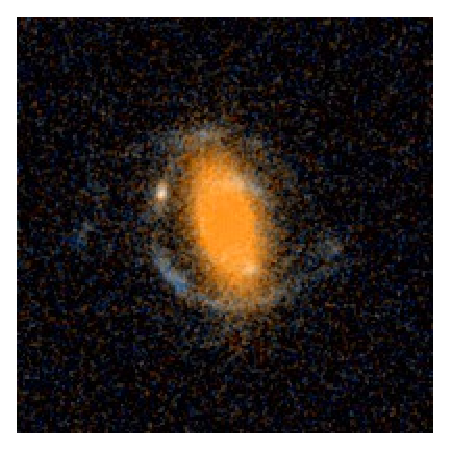
\includegraphics[width=0.9\linewidth]{figs/HSTJ135754_29-311509_1_sci.eps} 
\end{minipage}\hfill
\begin{minipage}{0.48\linewidth}
\centering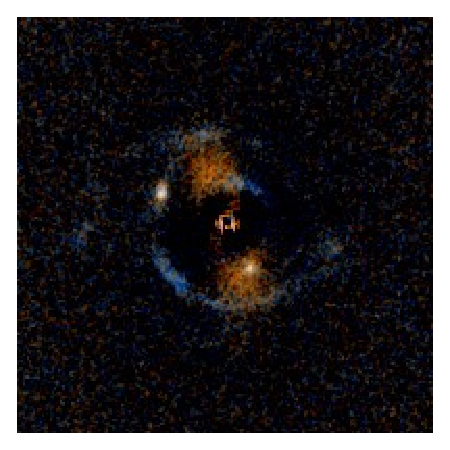
\includegraphics[width=0.9\linewidth]{figs/HSTJ135754_29-311509_1_sci_moffatdiff.eps} 
\end{minipage}
\caption{Left: HST image of gravitational lens \lens. Right:
automatic lens-subtracted version of this image. Images from
Marshall et al (in preparation).}
\label{fig:example}
\end{center}
\end{figure*}
%%%%%%%%%%%%%%%%%%%%%%%%%%%


%-------------------------------------------------------------------------------

\section{Paintings Generated by Zooniverse Users}
\label{sect:data}



%-------------------------------------------------------------------------------

\section{Analysis and Results}
\label{sect:results}

%%%%%%%%%%%%%%%%%%%%%%%%%%%
\begin{figure*}
\begin{center}
\centering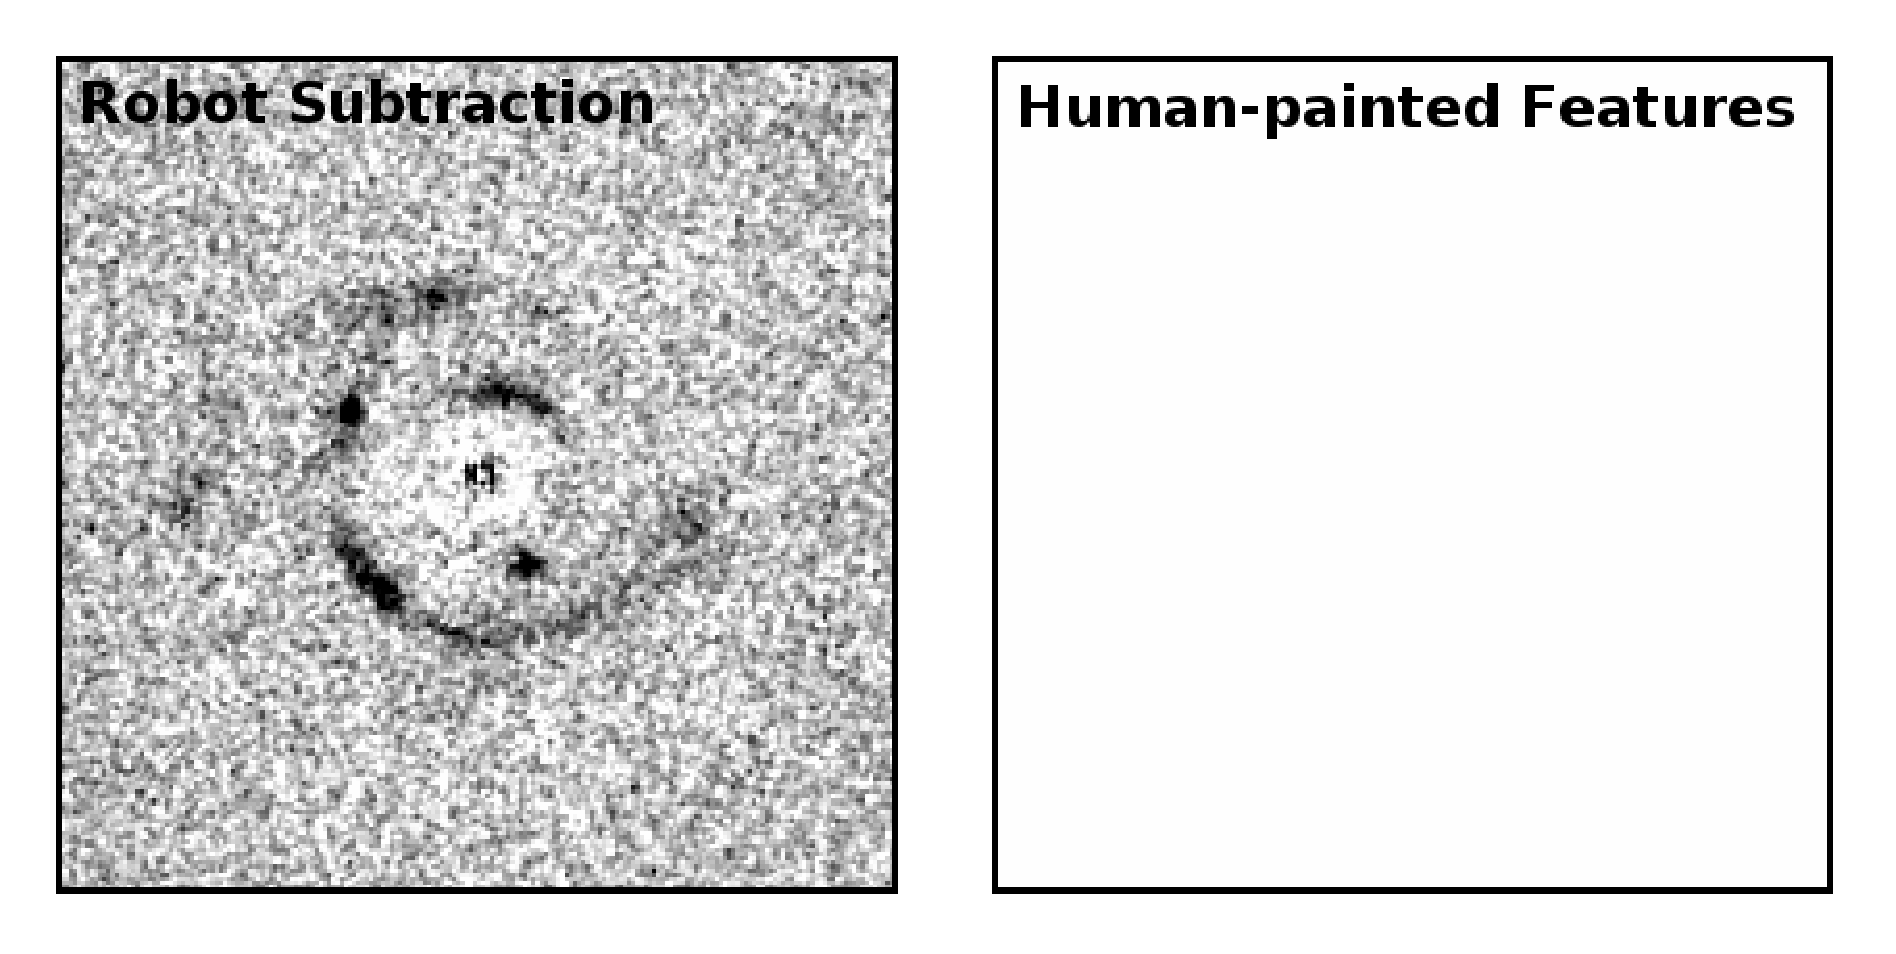
\includegraphics[width=\linewidth]{figs/machine-vs-painting_ds9.eps} 
\caption{Comparing the robotically subtracted HST/ACS F475W-band image (left) 
with the crowd-identified feature map (right).}
\label{fig:machine-vs-crowd}
\end{center}
\end{figure*}
%%%%%%%%%%%%%%%%%%%%%%%%%%%


%-------------------------------------------------------------------------------

\section{Conclusions}
\label{sect:concl}

From our simple analysis we draw the following conclusions:

\begin{enumerate}

\item The paintings done by citizen scientists span ... 

\item The mean (stacked) image and corresponding uncertainty map ... 

\end{enumerate}

%-----------------------------------------------------------------------

\section*{Acknowledgments} 

Painting on images for feature identification 
was conceived in discussions with the Zooniverse team in Oxford,
including Chris Lintott, Aprajita Verma, Arfon Smith and Rob Simpson. The
AstroTaches project was begun at the Dot Astronomy 3 meeting; we are grateful
to New College, Oxford, for providing the venue, and the conference organisers
for allowing us to hack the project together in an afternoon. 
%
% PJM received support from the Royal Society in the form of a research
% fellowship.                

%-------------------------------------------------------------------------------
\label{lastpage}

% \bibliography{references}

% MNRAS can be tricked into accepting bibtex but I forget how... 
% I used bubble to make a bbl file from our bib file:

% bubble -f astrotaches.tex references.bib 

% ==============================================================================

\documentclass[useAMS,usenatbib]{mn2e}

\usepackage[dvips]{graphicx}   % This is necessary to be able to include graphic
\usepackage{times}

\usepackage{epsfig}
\usepackage{amsmath,amssymb}
\usepackage{latexsym}
\usepackage{graphicx}% Include figure files
\usepackage{dcolumn}% Align table columns on decimal point
\usepackage{bm}% bold math
%\usepackage{epstopdf}

\def\reff@jnl#1{{\rm#1\/}}
\def\aj{\reff@jnl{AJ}}                  % Astronomical Journal
\def\araa{\reff@jnl{ARA\&A}}            % Annual Review of Astron and Astrophys
\def\apj{\reff@jnl{ApJ}}                % Astrophysical Journal
\def\apjl{\reff@jnl{ApJ}}               % Astrophysical Journal, Letters
\def\apjs{\reff@jnl{ApJS}}              % Astrophysical Journal, Supplement
\def\ao{\reff@jnl{Appl.Optics}}         % Applied Optics
\def\apss{\reff@jnl{Ap\&SS}}            % Astrophysics and Space Science
\def\aap{\reff@jnl{A\&A}}               % Astronomy and Astrophysics
\def\aapr{\reff@jnl{A\&A~Rev.}}         % Astronomy and Astrophysics Reviews
\def\aaps{\reff@jnl{A\&AS}}             % Astronomy and Astrophysics, Supplement
\def\azh{\reff@jnl{AZh}}                % Astronomicheskii Zhurnal
\def\baas{\reff@jnl{BAAS}}              % Bulletin of the AAS
\def\jrasc{\reff@jnl{JRASC}}            % Journal of the RAS of Canada
\def\memras{\reff@jnl{MmRAS}}           % Memoirs of the RAS
\def\mnras{\reff@jnl{MNRAS}}            % Monthly Notices of the RAS
\def\pra{\reff@jnl{Phys.Rev.A}}         % Physical Review A: General Physics
\def\prb{\reff@jnl{Phys.Rev.B}}         % Physical Review B: Solid State
\def\prc{\reff@jnl{Phys.Rev.C}}         % Physical Review C
\def\prd{\reff@jnl{Phys.Rev.D}}         % Physical Review D
\def\prl{\reff@jnl{Phys.Rev.Lett}}      % Physical Review Letters
\def\pasp{\reff@jnl{PASP}}              % Publications of the ASP
\def\pasj{\reff@jnl{PASJ}}              % Publications of the ASJ
\def\qjras{\reff@jnl{QJRAS}}            % Quarterly Journal of the RAS
\def\skytel{\reff@jnl{S\&T}}            % Sky and Telescope
\def\solphys{\reff@jnl{Solar~Phys.}}    % Solar Physics
\def\sovast{\reff@jnl{Soviet~Ast.}}     % Soviet Astronomy
\def\ssr{\reff@jnl{Space~Sci.Rev.}}     % Space Science Reviews
\def\zap{\reff@jnl{ZAp}}                % Zeitschrift fuer Astrophysik
\def\nat{\reff@jnl{Nature}}             % Nature 
\newcommand{\be}{\begin{equation}}
\newcommand{\ee}{\end{equation}}
\newcommand{\bea}{\begin{eqnarray}}
\newcommand{\eea}{\end{eqnarray}}
\newcommand{\bi}{\begin{itemize}}
\newcommand{\ei}{\end{itemize}}
% \newcommand\farcs{\mbox{$.\!\!^{\prime\prime}$}}
\def\vtr#1{{\bf #1}}
\def\mtx#1{{\bf #1}}

\def\lens{HST\,J135754.29$-$311509.1}

% ==============================================================================

\title%
[Astronomical Image Annotation]%
{AstroTaches: How Useful Are Annotative Paintings of Astronomical Images?}
\label{firstpage}

\author%
[Marshall et al]%
{Phil Marshall$^{1}$\thanks{E-mail:pjm@physics.ucsb.edu}, 
David W. Hogg$^{2}$,
Stuart R. Lowe$^{3}$
\newauthor Pamela L. Gay$^{4,5}$\\
$^{1}$Physics department, University of Oxford, \\
$^{2}$CCPP, NYU, New York, USA\\
$^{3}$Cardiff University, UK\\
$^{4}$Middle Illinois, USA\\
$^{5}$AstroSphere, USA}

\date{today}

\pagerange{\pageref{firstpage}--\pageref{lastpage}}

\pubyear{2011}

% ===============================================================================

\begin{document}

\maketitle

%-------------------------------------------------------------------------------

\begin{abstract}

Astronomical images can be complex, with the interesting features often
appearing at low signal to noise, or blended with other objects. Automated
methods for feature detection and deblending can fail if they are applied to
systems with unexpected features. In contrast,  human inspectors seem to learn
quickly what features are interesting, and identify them in confusing images.
In this work we investigate a web-based tool for ``painting'' over features in
astronomical images, and ask how useful these paintings are at summarising
interesting features. Specifically, we gathered, from members of the Galaxy
Zoo online user community, N paintings of the blue features in an HST image of
a gravitational lens. In a simple analysis of these paintings, we find...

\end{abstract}


\begin{keywords}
gravitational lensing --- surveys --- cosmology: observations
\end{keywords}


%-------------------------------------------------------------------------------

\section{Introduction}


%-------------------------------------------------------------------------------

\section{The AstroTaches Interface}
\label{sect:interface}



%-------------------------------------------------------------------------------

\section{A Simple Test Case: Gravitational Lens \lens}
\label{sect:testcase}


\begin{figure*}
\begin{center}
\begin{minipage}{0.48\linewidth}
\centering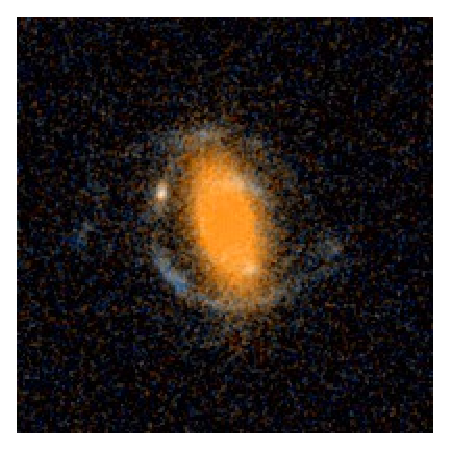
\includegraphics[width=0.9\linewidth]{figs/HSTJ135754_29-311509_1_sci.eps} 
\end{minipage}\hfill
\begin{minipage}{0.48\linewidth}
\centering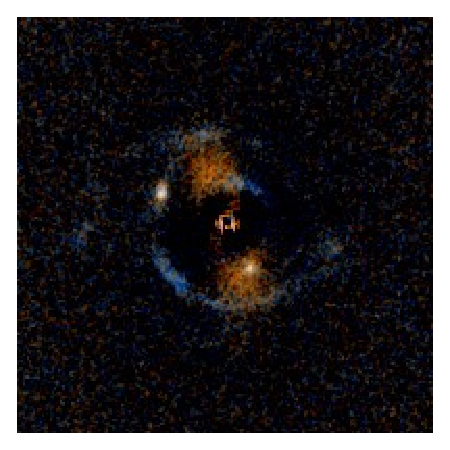
\includegraphics[width=0.9\linewidth]{figs/HSTJ135754_29-311509_1_sci_moffatdiff.eps} 
\end{minipage}
\caption{Left: HST image of gravitational lens \lens. Right:
automatic lens-subtracted version of this image. Images from
Marshall et al (in preparation).}
\label{fig:example}
\end{center}
\end{figure*}


%-------------------------------------------------------------------------------

\section{Paintings Generated by Zooniverse Users}
\label{sect:data}



%-------------------------------------------------------------------------------

\section{Analysis and Results}
\label{sect:results}



%-------------------------------------------------------------------------------

\section{Conclusions}
\label{sect:concl}

From our simple analysis we draw the following conclusions:

\begin{enumerate}

\item The paintings done by citizen scientists span ... 

\item The mean (stacked) image and corresponding uncertainty map ... 

\end{enumerate}

%-----------------------------------------------------------------------

\section*{Acknowledgments} 

Painting on images for feature identification 
was conceived in discussions with the Zooniverse team in Oxford,
including Chris Lintott, Aprajita Verma, Arfon Smith and Rob Simpson. The
AstroTaches project was begun at the Dot Astronomy 3 meeting; we are grateful
to New College, Oxford, for providing the venue, and the conference organisers
for allowing us to hack the project together in an afternoon. 
%
% PJM received support from the Royal Society in the form of a research
% fellowship.                

%-------------------------------------------------------------------------------
\label{lastpage}

% \bibliography{references}

% MNRAS can be tricked into accepting bibtex but I forget how... 
% I used bubble to make a bbl file from our bib file:

% bubble -f astrotaches.tex references.bib 

% ==============================================================================

\documentclass[useAMS,usenatbib]{mn2e}

\usepackage[dvips]{graphicx}   % This is necessary to be able to include graphic
\usepackage{times}

\usepackage{epsfig}
\usepackage{amsmath,amssymb}
\usepackage{latexsym}
\usepackage{graphicx}% Include figure files
\usepackage{dcolumn}% Align table columns on decimal point
\usepackage{bm}% bold math
%\usepackage{epstopdf}

\def\reff@jnl#1{{\rm#1\/}}
\def\aj{\reff@jnl{AJ}}                  % Astronomical Journal
\def\araa{\reff@jnl{ARA\&A}}            % Annual Review of Astron and Astrophys
\def\apj{\reff@jnl{ApJ}}                % Astrophysical Journal
\def\apjl{\reff@jnl{ApJ}}               % Astrophysical Journal, Letters
\def\apjs{\reff@jnl{ApJS}}              % Astrophysical Journal, Supplement
\def\ao{\reff@jnl{Appl.Optics}}         % Applied Optics
\def\apss{\reff@jnl{Ap\&SS}}            % Astrophysics and Space Science
\def\aap{\reff@jnl{A\&A}}               % Astronomy and Astrophysics
\def\aapr{\reff@jnl{A\&A~Rev.}}         % Astronomy and Astrophysics Reviews
\def\aaps{\reff@jnl{A\&AS}}             % Astronomy and Astrophysics, Supplement
\def\azh{\reff@jnl{AZh}}                % Astronomicheskii Zhurnal
\def\baas{\reff@jnl{BAAS}}              % Bulletin of the AAS
\def\jrasc{\reff@jnl{JRASC}}            % Journal of the RAS of Canada
\def\memras{\reff@jnl{MmRAS}}           % Memoirs of the RAS
\def\mnras{\reff@jnl{MNRAS}}            % Monthly Notices of the RAS
\def\pra{\reff@jnl{Phys.Rev.A}}         % Physical Review A: General Physics
\def\prb{\reff@jnl{Phys.Rev.B}}         % Physical Review B: Solid State
\def\prc{\reff@jnl{Phys.Rev.C}}         % Physical Review C
\def\prd{\reff@jnl{Phys.Rev.D}}         % Physical Review D
\def\prl{\reff@jnl{Phys.Rev.Lett}}      % Physical Review Letters
\def\pasp{\reff@jnl{PASP}}              % Publications of the ASP
\def\pasj{\reff@jnl{PASJ}}              % Publications of the ASJ
\def\qjras{\reff@jnl{QJRAS}}            % Quarterly Journal of the RAS
\def\skytel{\reff@jnl{S\&T}}            % Sky and Telescope
\def\solphys{\reff@jnl{Solar~Phys.}}    % Solar Physics
\def\sovast{\reff@jnl{Soviet~Ast.}}     % Soviet Astronomy
\def\ssr{\reff@jnl{Space~Sci.Rev.}}     % Space Science Reviews
\def\zap{\reff@jnl{ZAp}}                % Zeitschrift fuer Astrophysik
\def\nat{\reff@jnl{Nature}}             % Nature 
\newcommand{\be}{\begin{equation}}
\newcommand{\ee}{\end{equation}}
\newcommand{\bea}{\begin{eqnarray}}
\newcommand{\eea}{\end{eqnarray}}
\newcommand{\bi}{\begin{itemize}}
\newcommand{\ei}{\end{itemize}}
% \newcommand\farcs{\mbox{$.\!\!^{\prime\prime}$}}
\def\vtr#1{{\bf #1}}
\def\mtx#1{{\bf #1}}

\def\lens{HST\,J135754.29$-$311509.1}

% ==============================================================================

\title%
[Astronomical Image Annotation]%
{AstroTaches: How Useful Are Annotative Paintings of Astronomical Images?}
\label{firstpage}

\author%
[Marshall et al]%
{Phil Marshall$^{1}$\thanks{E-mail:pjm@physics.ucsb.edu}, 
David W. Hogg$^{2}$,
Stuart R. Lowe$^{3}$
\newauthor Pamela L. Gay$^{4,5}$\\
$^{1}$Physics department, University of Oxford, \\
$^{2}$CCPP, NYU, New York, USA\\
$^{3}$Cardiff University, UK\\
$^{4}$Middle Illinois, USA\\
$^{5}$AstroSphere, USA}

\date{today}

\pagerange{\pageref{firstpage}--\pageref{lastpage}}

\pubyear{2011}

% ===============================================================================

\begin{document}

\maketitle

%-------------------------------------------------------------------------------

\begin{abstract}

Astronomical images can be complex, with the interesting features often
appearing at low signal to noise, or blended with other objects. Automated
methods for feature detection and deblending can fail if they are applied to
systems with unexpected features. In contrast,  human inspectors seem to learn
quickly what features are interesting, and identify them in confusing images.
In this work we investigate a web-based tool for ``painting'' over features in
astronomical images, and ask how useful these paintings are at summarising
interesting features. Specifically, we gathered, from members of the Galaxy
Zoo online user community, N paintings of the blue features in an HST image of
a gravitational lens. In a simple analysis of these paintings, we find...

\end{abstract}


\begin{keywords}
gravitational lensing --- surveys --- cosmology: observations
\end{keywords}


%-------------------------------------------------------------------------------

\section{Introduction}


%-------------------------------------------------------------------------------

\section{The AstroTaches Interface}
\label{sect:interface}



%-------------------------------------------------------------------------------

\section{A Simple Test Case: Gravitational Lens \lens}
\label{sect:testcase}


\begin{figure*}
\begin{center}
\begin{minipage}{0.48\linewidth}
\centering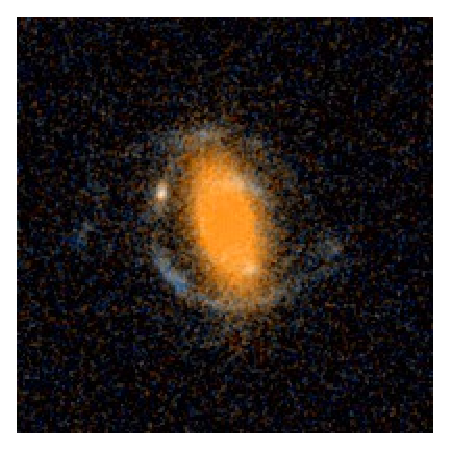
\includegraphics[width=0.9\linewidth]{figs/HSTJ135754_29-311509_1_sci.eps} 
\end{minipage}\hfill
\begin{minipage}{0.48\linewidth}
\centering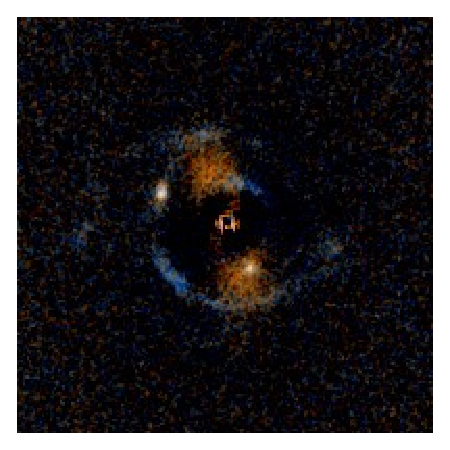
\includegraphics[width=0.9\linewidth]{figs/HSTJ135754_29-311509_1_sci_moffatdiff.eps} 
\end{minipage}
\caption{Left: HST image of gravitational lens \lens. Right:
automatic lens-subtracted version of this image. Images from
Marshall et al (in preparation).}
\label{fig:example}
\end{center}
\end{figure*}


%-------------------------------------------------------------------------------

\section{Paintings Generated by Zooniverse Users}
\label{sect:data}



%-------------------------------------------------------------------------------

\section{Analysis and Results}
\label{sect:results}



%-------------------------------------------------------------------------------

\section{Conclusions}
\label{sect:concl}

From our simple analysis we draw the following conclusions:

\begin{enumerate}

\item The paintings done by citizen scientists span ... 

\item The mean (stacked) image and corresponding uncertainty map ... 

\end{enumerate}

%-----------------------------------------------------------------------

\section*{Acknowledgments} 

Painting on images for feature identification 
was conceived in discussions with the Zooniverse team in Oxford,
including Chris Lintott, Aprajita Verma, Arfon Smith and Rob Simpson. The
AstroTaches project was begun at the Dot Astronomy 3 meeting; we are grateful
to New College, Oxford, for providing the venue, and the conference organisers
for allowing us to hack the project together in an afternoon. 
%
% PJM received support from the Royal Society in the form of a research
% fellowship.                

%-------------------------------------------------------------------------------
\label{lastpage}

% \bibliography{references}

% MNRAS can be tricked into accepting bibtex but I forget how... 
% I used bubble to make a bbl file from our bib file:

% bubble -f astrotaches.tex references.bib 

% ==============================================================================

\documentclass[useAMS,usenatbib]{mn2e}

\usepackage[dvips]{graphicx}   % This is necessary to be able to include graphic
\usepackage{times}

\usepackage{epsfig}
\usepackage{amsmath,amssymb}
\usepackage{latexsym}
\usepackage{graphicx}% Include figure files
\usepackage{dcolumn}% Align table columns on decimal point
\usepackage{bm}% bold math
%\usepackage{epstopdf}

\def\reff@jnl#1{{\rm#1\/}}
\def\aj{\reff@jnl{AJ}}                  % Astronomical Journal
\def\araa{\reff@jnl{ARA\&A}}            % Annual Review of Astron and Astrophys
\def\apj{\reff@jnl{ApJ}}                % Astrophysical Journal
\def\apjl{\reff@jnl{ApJ}}               % Astrophysical Journal, Letters
\def\apjs{\reff@jnl{ApJS}}              % Astrophysical Journal, Supplement
\def\ao{\reff@jnl{Appl.Optics}}         % Applied Optics
\def\apss{\reff@jnl{Ap\&SS}}            % Astrophysics and Space Science
\def\aap{\reff@jnl{A\&A}}               % Astronomy and Astrophysics
\def\aapr{\reff@jnl{A\&A~Rev.}}         % Astronomy and Astrophysics Reviews
\def\aaps{\reff@jnl{A\&AS}}             % Astronomy and Astrophysics, Supplement
\def\azh{\reff@jnl{AZh}}                % Astronomicheskii Zhurnal
\def\baas{\reff@jnl{BAAS}}              % Bulletin of the AAS
\def\jrasc{\reff@jnl{JRASC}}            % Journal of the RAS of Canada
\def\memras{\reff@jnl{MmRAS}}           % Memoirs of the RAS
\def\mnras{\reff@jnl{MNRAS}}            % Monthly Notices of the RAS
\def\pra{\reff@jnl{Phys.Rev.A}}         % Physical Review A: General Physics
\def\prb{\reff@jnl{Phys.Rev.B}}         % Physical Review B: Solid State
\def\prc{\reff@jnl{Phys.Rev.C}}         % Physical Review C
\def\prd{\reff@jnl{Phys.Rev.D}}         % Physical Review D
\def\prl{\reff@jnl{Phys.Rev.Lett}}      % Physical Review Letters
\def\pasp{\reff@jnl{PASP}}              % Publications of the ASP
\def\pasj{\reff@jnl{PASJ}}              % Publications of the ASJ
\def\qjras{\reff@jnl{QJRAS}}            % Quarterly Journal of the RAS
\def\skytel{\reff@jnl{S\&T}}            % Sky and Telescope
\def\solphys{\reff@jnl{Solar~Phys.}}    % Solar Physics
\def\sovast{\reff@jnl{Soviet~Ast.}}     % Soviet Astronomy
\def\ssr{\reff@jnl{Space~Sci.Rev.}}     % Space Science Reviews
\def\zap{\reff@jnl{ZAp}}                % Zeitschrift fuer Astrophysik
\def\nat{\reff@jnl{Nature}}             % Nature 
\newcommand{\be}{\begin{equation}}
\newcommand{\ee}{\end{equation}}
\newcommand{\bea}{\begin{eqnarray}}
\newcommand{\eea}{\end{eqnarray}}
\newcommand{\bi}{\begin{itemize}}
\newcommand{\ei}{\end{itemize}}
% \newcommand\farcs{\mbox{$.\!\!^{\prime\prime}$}}
\def\vtr#1{{\bf #1}}
\def\mtx#1{{\bf #1}}

\def\lens{HST\,J135754.29$-$311509.1}

% ==============================================================================

\title%
[Astronomical Image Annotation]%
{AstroTaches: How Useful Are Annotative Paintings of Astronomical Images?}
\label{firstpage}

\author%
[Marshall et al]%
{Phil Marshall$^{1}$\thanks{E-mail:pjm@physics.ucsb.edu}, 
David W. Hogg$^{2}$,
Stuart R. Lowe$^{3}$
\newauthor Pamela L. Gay$^{4,5}$\\
$^{1}$Physics department, University of Oxford, \\
$^{2}$CCPP, NYU, New York, USA\\
$^{3}$Cardiff University, UK\\
$^{4}$Middle Illinois, USA\\
$^{5}$AstroSphere, USA}

\date{today}

\pagerange{\pageref{firstpage}--\pageref{lastpage}}

\pubyear{2011}

% ===============================================================================

\begin{document}

\maketitle

%-------------------------------------------------------------------------------

\begin{abstract}

Astronomical images can be complex, with the interesting features often
appearing at low signal to noise, or blended with other objects. Automated
methods for feature detection and deblending can fail if they are applied to
systems with unexpected features. In contrast,  human inspectors seem to learn
quickly what features are interesting, and identify them in confusing images.
In this work we investigate a web-based tool for ``painting'' over features in
astronomical images, and ask how useful these paintings are at summarising
interesting features. Specifically, we gathered, from members of the Galaxy
Zoo online user community, N paintings of the blue features in an HST image of
a gravitational lens. In a simple analysis of these paintings, we find...

\end{abstract}


\begin{keywords}
gravitational lensing --- surveys --- cosmology: observations
\end{keywords}


%-------------------------------------------------------------------------------

\section{Introduction}


%-------------------------------------------------------------------------------

\section{The AstroTaches Interface}
\label{sect:interface}



%-------------------------------------------------------------------------------

\section{A Simple Test Case: Gravitational Lens \lens}
\label{sect:testcase}


\begin{figure*}
\begin{center}
\begin{minipage}{0.48\linewidth}
\centering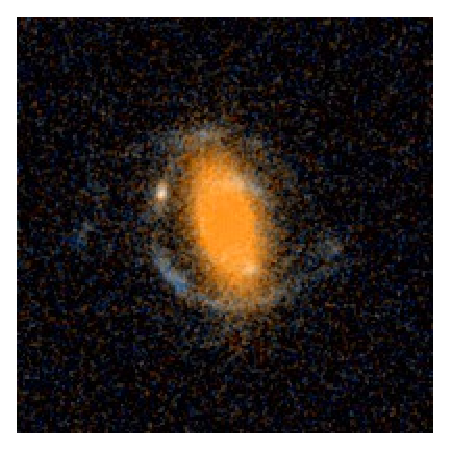
\includegraphics[width=0.9\linewidth]{figs/HSTJ135754_29-311509_1_sci.eps} 
\end{minipage}\hfill
\begin{minipage}{0.48\linewidth}
\centering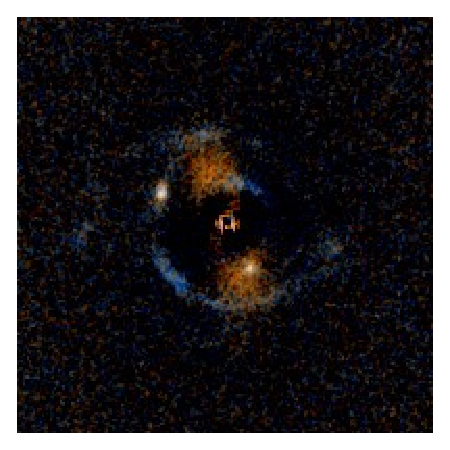
\includegraphics[width=0.9\linewidth]{figs/HSTJ135754_29-311509_1_sci_moffatdiff.eps} 
\end{minipage}
\caption{Left: HST image of gravitational lens \lens. Right:
automatic lens-subtracted version of this image. Images from
Marshall et al (in preparation).}
\label{fig:example}
\end{center}
\end{figure*}


%-------------------------------------------------------------------------------

\section{Paintings Generated by Zooniverse Users}
\label{sect:data}



%-------------------------------------------------------------------------------

\section{Analysis and Results}
\label{sect:results}



%-------------------------------------------------------------------------------

\section{Conclusions}
\label{sect:concl}

From our simple analysis we draw the following conclusions:

\begin{enumerate}

\item The paintings done by citizen scientists span ... 

\item The mean (stacked) image and corresponding uncertainty map ... 

\end{enumerate}

%-----------------------------------------------------------------------

\section*{Acknowledgments} 

Painting on images for feature identification 
was conceived in discussions with the Zooniverse team in Oxford,
including Chris Lintott, Aprajita Verma, Arfon Smith and Rob Simpson. The
AstroTaches project was begun at the Dot Astronomy 3 meeting; we are grateful
to New College, Oxford, for providing the venue, and the conference organisers
for allowing us to hack the project together in an afternoon. 
%
% PJM received support from the Royal Society in the form of a research
% fellowship.                

%-------------------------------------------------------------------------------
\label{lastpage}

% \bibliography{references}

% MNRAS can be tricked into accepting bibtex but I forget how... 
% I used bubble to make a bbl file from our bib file:

% bubble -f astrotaches.tex references.bib 

\input{mn.bbl}

\bsp
%-------------------------------------------------------------------------------
\end{document}
% ==============================================================================


\bsp
%-------------------------------------------------------------------------------
\end{document}
% ==============================================================================


\bsp
%-------------------------------------------------------------------------------
\end{document}
% ==============================================================================


\bsp
%-------------------------------------------------------------------------------
\end{document}
% ==============================================================================
